\section{Experimental Results}
\label{Experimental Results}

We used the simulator to examine the results of the game between the adversary and the utility described in Section \ref{Game}. We examined the effectiveness of the four adverserial strategies and the corresponding defense mechanisms presented earlier (Table \ref{strategies}). In the first scenario, there are an equal number of each class of customer. In the second, 40\% are Bakeries, 40\% are Batteries, and the remaining 20\% are Buckets. In both scenarios, we assume that the attacker and the utility have the same budget, \ie they can attack or defend the same number of customers. All of our results are over 15,000 total customers. The results presented here are averaged over 10 different random number seeds in order to eliminate any bias in a given sample from the distributions. 
The metric that we are interested in is the mismatch between the supply and the demand at the utility, summed up over all the time steps of the simulation (we had 100 time steps for these results). A greater mismatch means worse impact of the attack. We provide the result as percentage change from the baseline, which is the case with no attack. So a greater change means a worse result. 

\begin{figure*}[htp]
    \centering
    \subfigure[Scenario 1: Equal proportion of load types - Bakeries, Batteries, and Buckets]{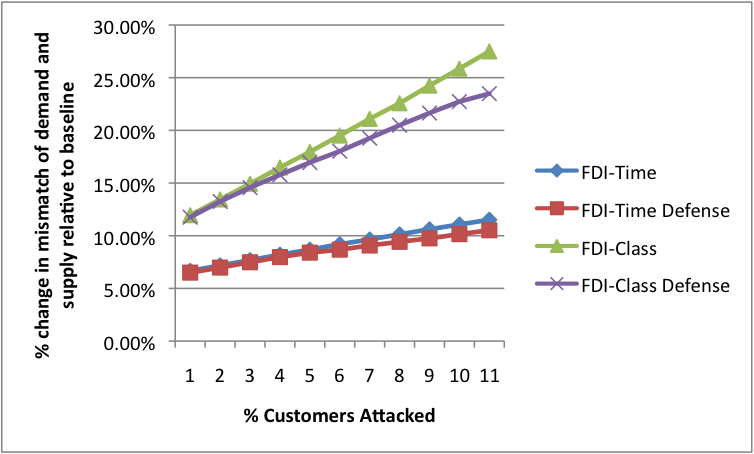
\includegraphics[width=.5\textwidth]{naieve-equal-attacks.png}}\hfill
    \subfigure[Scenario 2: 40\% Bakeries, 40\% Batteries, 20\% Buckets]{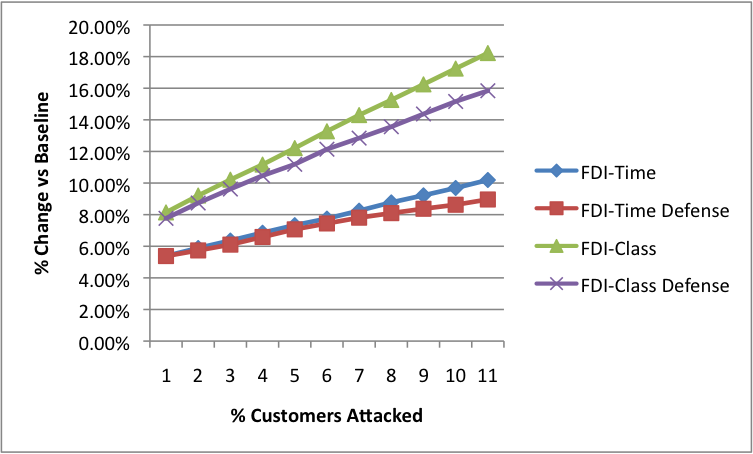
\includegraphics[width=.5\textwidth]{naieve-unequal-attacks.png}}  
    \caption{Results for the Na\"\i ve Adversary}
    \label{naive}  
\end{figure*}

We first considered a na\"\i ve adversary who picks from among all the customers in a uniform random manner. To even the scales, we also had the utility choose assets to defend in a uniform random manner. In this case neither the Jamming nor the FDI-Load attack had any significant effect, and so are omitted from Figure \ref{naive}. Our defense is relatively ineffective against the na\"\i ve attacker, because of the random choices made by the adversary. However, the attack itself is also far less effective: only increasing the mismatch by 28\% in the worst case versus 52\% for the strategic adversary. The FDI-Class attack is more effective than the FDI-Time attack underlining how important the flexibility of buckets is to the utility for its load scheduling. 

Given this na\"\i ve baseline, we examined how much more effective a \emph{strategic} adversary is. In particular, the adversary preferentially targets the loads that have higher flexibility. In our simulation setting, this leads to the situation that only bakeries are targeted for all attacks other than the FDI-Class where it converts some buckets into bakeries. Figure \ref{strategic} show.

\begin{figure*}[htp]
    \centering
    \subfigure[Scenario 1: Equal proportion of load types - Bakeries, Batteries, and Buckets]{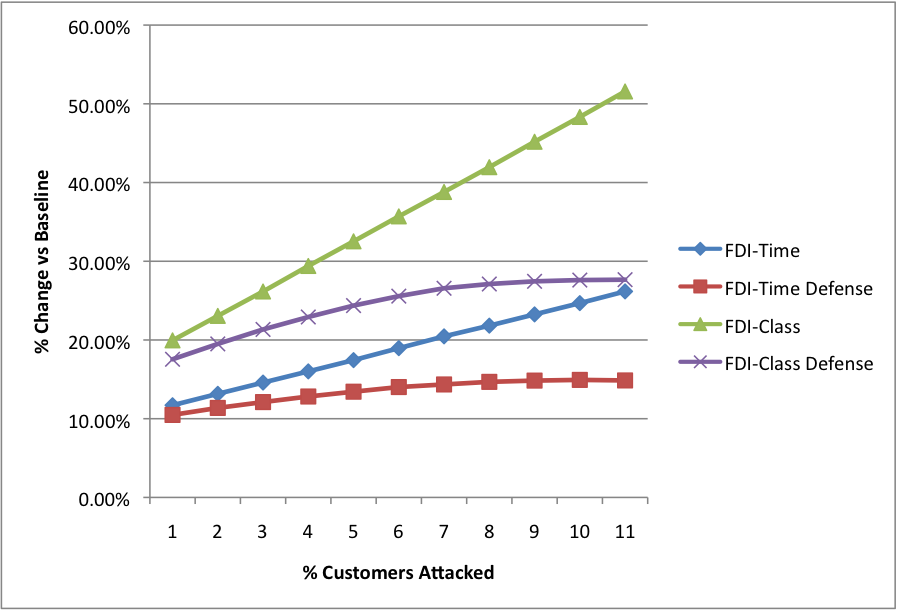
\includegraphics[width=.48\textwidth]{equal-attacks.png}}\hfill
    \subfigure[Scenario 2: 40\% Bakeries, 40\% Batteries, 20\% Buckets]{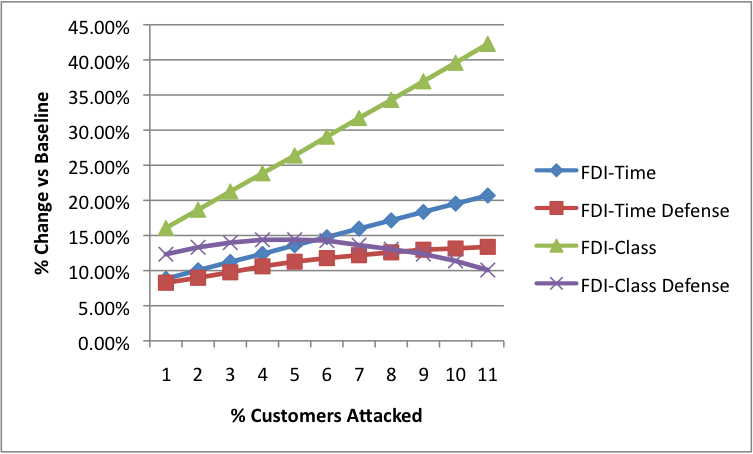
\includegraphics[width=.52\textwidth]{unequal-attacks.png}}  
    \caption{Results for the Strategic Adversary}
    \label{strategic}  
\end{figure*}

Again, the FDI-Load and Jam attacks are not effective, and are omitted from our results. This means that the low level of FDI-Load to remain stealthy makes it such that existing scheduling is not perturbed by it. However, the strategic attacks, FDI-Class and FDI-Time, have a significant impact, increasing mismatch by 52\% in the worst case. However, our defense was able to blunt the strategic adversary back down to the efficacy of the na\"\i ve, random adversary. This is a significant decrease: dropping the attacker induced mismatch from 52\% to 28\% of baseline. 
The other notable result is that the efficacy of our defense against the FDI-Class attack \emph{increases} as more customers are attacked. This attack targets Buckets, the most flexible type of customer, and turns them into Bakeries, the least. The efficacy of our defense, which preserves Buckets, underscores the critical nature of the flexibility they provide to the utility. 

